\chapter{Perancangan}
\label{chap:perancangan}

Pada bab ini dijelaskan mengenai beberapa perancangan yang dilakukan dalam penelitian ini yaitu rancangan kelas dan rancangan antarmuka pengguna

\section{Rancangan Kelas}
Berdasarkan hasil analisis dari masalah yang dihadapi, dibentuklah diagram kelas pada gambar \ref{fig:diagramkelas} sebagai gambaran dari perangkat lunak yang akan dibuat.

\subsection{\textit{Document}}

\begin{figure}[h]
	\begin{center}
		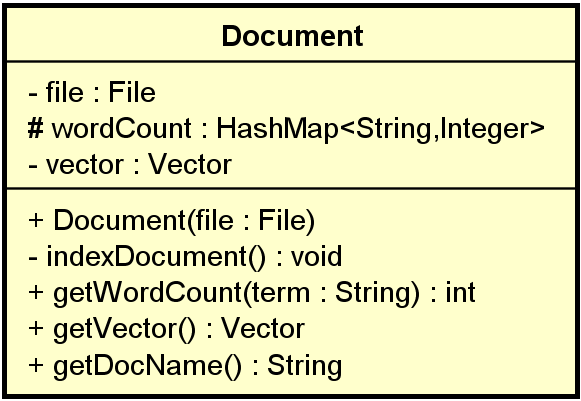
\includegraphics[width=0.5\textwidth]{DiagramKelas/Document}
		\caption{Kelas \textit{Document}}
		\label{fig:kelasDocument}
	\end{center}
\end{figure}

Kelas ini merupakan representasi dari dokumen yang akan diproses dalam pengelompokan. Kelas ini berfungsi untuk menyimpan informasi yang dibutuhkan dari sebuah dokumen selama proses pengelompokan. Atribut yang dimiliki oleh kelas \textit{Document} adalah:

\begin{itemize}
	\item \textit{wordCount}: bertipe \textit{HashMap} dengan \textit{key} bertipe \textit{String} dan \textit{value} bertipe \textit{Integer}. Atribut ini menyimpan pasangan kata yang dimiliki oleh dokumen tersebut dan frekuensinya.
	\item \textit{file}: atribut ini bertipe \textit{File} milik \textit{package} java.io yang berfungsi untuk merepresentasikan \textit{file} dari dokumen yang akan diproses.
	\item \textit{vector}: atribut bertipe \textit{VectorSpaceModel} ini merepresentasikan model ruang vektor pada sebuah dokumen.
\end{itemize}

\textit{Method} yang terdapat dalam kelas ini adalah:

\begin{itemize}
	\item \textit{Document}: merupakan \textit{constructor} dengan sebuah parameter bertipe \textit{File} yaitu \textit{file} dari dokumen yang akan dikelompokkan.
	\item \textit{indexDocument}: \textit{method} tanpa kembalian (\textit{void}) yang berfungsi untuk mengindeks dokumen untuk mengisi atribut \textit{wordCount}.
	\item \textit{getWordCount}: berfungsi untuk mengembalikan banyaknya istilah \textit{term} muncul dalam dokumen.
	\item \textit{getVector}: merupakan \textit{getter} dari variabel \textit{vector}.
	\item \textit{determineClusterCode}: berfungsi untuk menentukan \textit{cluster} dari dokumen.
	\item \textit{getDocName}: mengembalikan nama \textit{file} dari dokumen.
\end{itemize}

\subsection{\textit{VectorSpaceModel}}

\begin{figure}[h]
	\begin{center}
		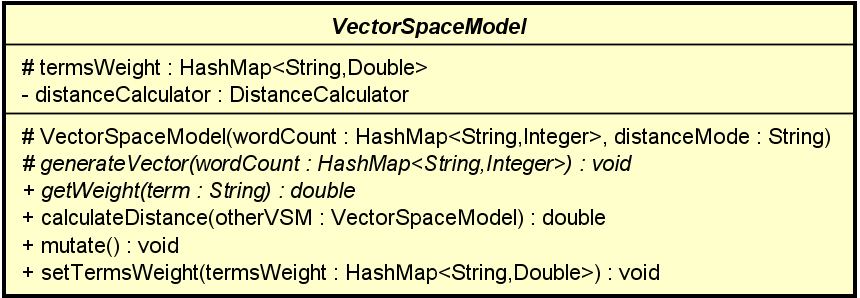
\includegraphics[width=0.5\textwidth]{DiagramKelas/VectorSpaceModel}
		\caption{Kelas \textit{VectorSpaceModel}}
		\label{fig:kelasVSM}
	\end{center}
\end{figure}

Kelas ini merupakan kelas abstrak yang merepresentasikan model ruang vektor. kelas ini memiliki fungsi-fungsi yang umum dimiliki oleh sebuah model ruang vektor. Atribut yang dimiliki kelas ini adalah:

\begin{itemize}
	\item \textit{termsWeight}: bertipe \textit{Hashmap} dengan \textit{key} berupa \textit{String} dan \textit{value} berupa \textit{Double}. atribut ini menyimpan pasangan istilah dan bebatnya sesuai dengan metode pembobotan.
	\item \textit{distanceCalculator}: bertipe \textit{DistanceCalculator} dan merupakan objek yang akan digunakan untuk menghitung jarak antar vektor.
\end{itemize}

\textit{Method} yang terdapat dalam kelas ini adalah:

\begin{itemize}
	\item \textit{VectorSpaceModel}: merupakan constructor dengan dua parameter yaitu \textit{wordCount} bertipe \textit{Hashmap<String,Integer>} yang merupakan pasangan kata dan banyak kemunculannya dalam dokumen serta \textit{distanceMode} bertipe \textit{String} yang akan menentukan tipe perhitungan jarak antar vektor.
	\item \textit{generateVector}: merupakan \textit{method} tanpa parameter untuk mengubah banyak kemunculan kata menjadi berat.
	\item \textit{getWeight}: berfungsi untuk mengembalikan berat dari istilah \textit{term}.
	\item \textit{calculateDistance}: berfungsi untuk menghitung jarak antara vektor ini dengan \textit{otherVSM} menggunakan metode yang dipilih pada parameter di \textit{constructor}.
	\item \textit{mutate}: merupakan \textit{method} untuk melakukan mutasi pada sebuah dimensi dalam vektor.
	\item \textit{setTermsWeight}: merupakan setter dari atribut \textit{termsWeight}.
\end{itemize}

\subsection{\textit{BagOfWordVSM}}

\begin{figure}[h]
	\begin{center}
		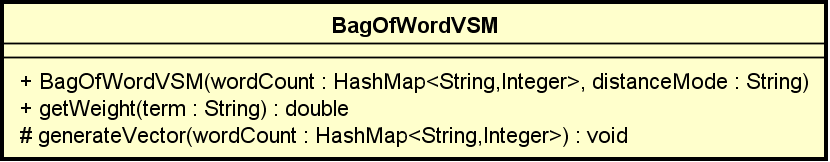
\includegraphics[width=0.5\textwidth]{DiagramKelas/BagOfWordVSM}
		\caption{Kelas \textit{BagOfWordVSM}}
		\label{fig:kelasBagOfWordVSM}
	\end{center}
\end{figure}

Kelas ini merupakan kelas yang mengimplementasikan kelas \textit{VectorSpaceModel}. Kelas ini menggunakan metode pembobotan \textit{BagOfWord} di mana bobot tiap istilah merupakan banyaknya kemunculan istilah itu sendiri. Atribut yang dimiliki kelas ini seluruhnya merupakan atribut yang diturunkan dari kelas \textit{VectorSpaceModel} dan hanya melakukan \textit{override} pada \textit{method} yang masih bersifat abstrak.

\subsection{\textit{DistanceCalculator}}

\begin{figure}[h]
	\begin{center}
		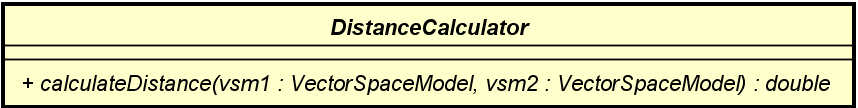
\includegraphics[width=0.5\textwidth]{DiagramKelas/DistanceCalculator}
		\caption{Kelas \textit{DistanceCalculator}}
		\label{fig:kelasDistanceCalculator}
	\end{center}
\end{figure}

Kelas ini merupakan kelas abstrak yang berfungsi untuk menghitung jarak antara dua buah objek bertipe \textit{VectorSpaceModel}. Kelas ini tidak memiliki atribut dan hanya memiliki sebuah \textit{method} abstrak yaitu \textit{calculateDistance} yang memiliki dua buah parameter \textit{vsm1} dan \textit{vsm2}. Hasil yang dikembalikan oleh \textit{method} ini adalah jarak dari kedua vektor tersebut sesuai dengan metode perhitungan jaraknya.

\subsection{\textit{EuclideanDistanceCalculator}}

\begin{figure}[h]
	\begin{center}
		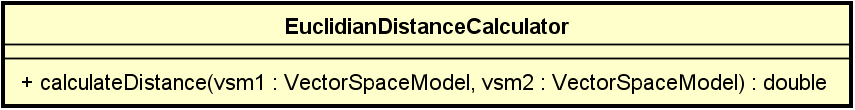
\includegraphics[width=0.5\textwidth]{DiagramKelas/EuclideanDistanceCalculator}
		\caption{Kelas \textit{EuclideanDistanceCalculator}}
		\label{fig:kelasEuclideanDist}
	\end{center}
\end{figure}

Kelas ini mengimplementasikan kelas abstrak \textit{DistanceCalculator}. Kelas ini hanya melakukan \textit{override} pada \textit{method calculateDistance} dengan melakukan perhitungan menggunakan jarak euclidean untuk menghitung jarak antara dua buah vektor (Subbab \ref{sub:euclideanDist}).

\subsection{\textit{CosineDistanceCalculator}}

\begin{figure}[h]
	\begin{center}
		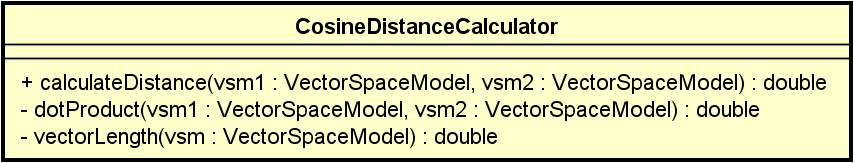
\includegraphics[width=0.5\textwidth]{DiagramKelas/CosineDistanceCalculator}
		\caption{Kelas \textit{CosineDistanceCalculator}}
		\label{fig:kelasCosineDist}
	\end{center}
\end{figure}

Kelas ini juga mengimplementasikan kelas abstrak \textit{DistanceCalculator}. Kelas ini memiliki dua \textit{method} tambahan selain melakukan \textit{override} pada \textit{method calculateDistance}. \textit{Method} yang ada pada kelas ini adalah:

\begin{itemize}
	\item \textit{calculateDistance}: merupakan \textit{method} yang diturunkan dari kelas \textit{DistanceCalculator}. \textit{Method} ini mengembalikan jarak dari \textit{vsm1} dan \textit{vsm2} yang dihitung menggunakan persamaan cosinus (Subbab \ref{sub:cosineDist}).
	\item \textit{dotProduct}: berfungsi untuk menghitung hasil perkalian titik (\textit{dot product}) antara \textit{vsm1} dan \textit{vsm 2}.
	\item \textit{vectorLength}: berfungsi untuk menghitung panjang dari vektor \textit{vsm}.
\end{itemize}

\subsection{\textit{Dictionary}}

\begin{figure}[h]
	\begin{center}
		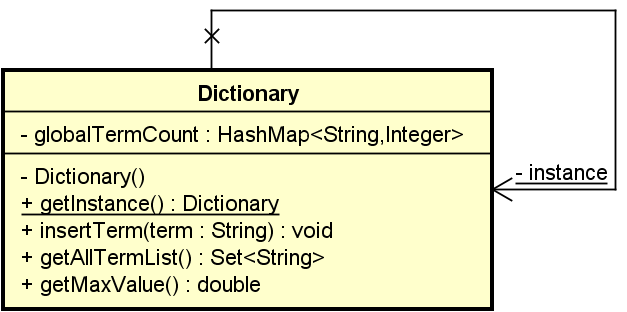
\includegraphics[width=0.5\textwidth]{DiagramKelas/Dictionary}
		\caption{Kelas \textit{Dictionary}}
		\label{fig:kelasDictionary}
	\end{center}
\end{figure}

Kelas ini merepresentasikan sebuah kamus yang menangani seluruh kebutuhan dalam proses pengelompokan yang membutuhkan akses global untuk keseluruhan koleksi dokumen. Atribut yang ada dalam kelas ini adalah:

\begin{itemize}
	\item \textit{globalTermCount}: bertipe \textit{HashMap} dengan \textit{key} bertipe \textit{String} dan \textit{value} bertipe \textit{Integer}. Atribut ini berfungsi untuk menyimpan seluruh istilah yang muncul dan banyak kemunculannya dalam keseluruhan koleksi dokumen.
	\item \textit{instance}: merupakan objek bertipe \textit{Dictionary} sebagai instansiasi satu-satunya dari kelas \textit{Dictionary} karena kelas ini bersifat \textit{singleton}.
\end{itemize}

\textit{Method} yang ada pada kelas ini adalah:

\begin{itemize}
	\item \textit{Dictionary}: merupakan \textit{constructor private} untuk menjamin tidak akan ada lebih dari satu \textit{instance} selama perangkat lunak berjalan.
	\item \textit{getInstance}: merupakan \textit{method static} yang berfungsi sebagai \textit{getter} dari atribut \textit{instance}.
	\item \textit{insertTerm}: berfungsi untuk memasukkan istilah \textit{term} ke dalam variabel \textit{globalTermCount}.
	\item \textit{getAllTermList}: bertugas mengembalikan daftar seluruh istilah yang pernah muncul di seluruh koleksi dokumen.
	\item \textit{getValue}: bertugas mengembalikan banyaknya kata \textit{term} muncul dalam seluruh koleksi dokumen. 
\end{itemize}

\subsection{\textit{Gene}}

\begin{figure}[h]
	\begin{center}
		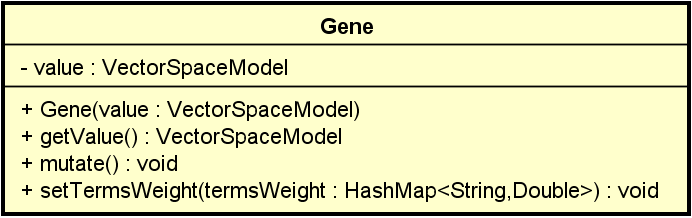
\includegraphics[width=0.5\textwidth]{DiagramKelas/Gene}
		\caption{Kelas \textit{Gene}}
		\label{fig:kelasGene}
	\end{center}
\end{figure}

Kelas ini merepresentasikan gen dalam algoritma genetika. Kelas ini hanya memiliki sebuah atribut \textit{value} bertipe \textit{VectorSpaceModel}. Atribut ini menyimpan model ruang vektor yang menjadi titik pusat \textit{cluster} (\textit{centroid}). \textit{Method} yang ada pada kelas ini adalah:

\begin{itemize}
	\item \textit{Gene}: merupakan \textit{constructor} dari kelas \textit{Gene} yang membutuhkan sebuah parameter bertipe \textit{VectorSpaceModel} untuk mengisi variabel \textit{value}.
	\item \textit{getValue}: merupakan \textit{getter} dari atribut \textit{value}.
	\item \textit{mutate}: berfungsi untuk melakukan mutasi pada gen. \textit{Method} ini sebenarnya hanya bertugas memanggil fungsi \textit{mutate()} dari atribut \textit{value}.
	\item \textit{setTermsWeight}: berfungsi untuk mengubah nilai atribut \textit{termsWeight} milik atribut \textit{value}.
\end{itemize}

\subsection{\textit{Chromosome}}

\begin{figure}[h]
	\begin{center}
		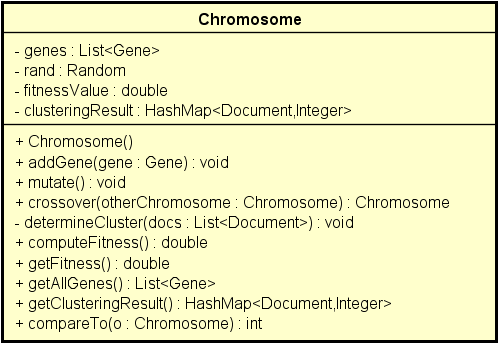
\includegraphics[width=0.5\textwidth]{DiagramKelas/Chromosome}
		\caption{Kelas \textit{Chromosome}}
		\label{fig:kelasChromosome}
	\end{center}
\end{figure}

Kelas ini merepresentasikan kromosom dalam algoritma genetika (Subbab \ref{sub:chromosome}). Atribut yang terdapat dalam kelas ini adalah:

\begin{itemize}
	\item \textit{genes}: bertipe \textit{List of Gene} dan merupakan kumpulan gen yang terdapat dalam kromosom.
	\item \textit{MUTATION\_ PROBABILITY}: merupakan atribut yang bersifat \textit{static} dan \textit{final} yang berisi probabilitas terjadinya mutasi dalam proses pembangkitan keturunan.
\end{itemize}

\textit{Method} yang terdapat dalam kelas ini adalah:

\begin{itemize}
	\item \textit{Chromosome}: merupakan \textit{constructor} tanpa parameter untuk membentuk objek dari kelas \textit{Chromosome}.
	\item \textit{addGene}: bertugas untuk menambahkan satu gen ke dalam kromosom (ke dalam atribut \textit{genes}).
	\item \textit{mutate}: berfungsi untuk melakukan mutasi pada kromosom dengan cara melakukan mutasi pada sebuah gen secara acak (Subbab \ref{sub:mutation}).
	\item \textit{crossover}: bertugas untuk melakukan persilangan dengan kromosom lain untuk mengahsilkan keturunan (Subbab \ref{sub:crossover}).
	\item \textit{computeFitness}: mengembalikan nilai \textit{fitness} dari kromosom (Subbab \ref{sub:fitnessFn}).
	\item \textit{getAllGenes}: merupakan \textit{getter} dari atribut \textit{genes}.
\end{itemize}

\subsection{\textit{Clusterer}}

\begin{figure}[h]
	\begin{center}
		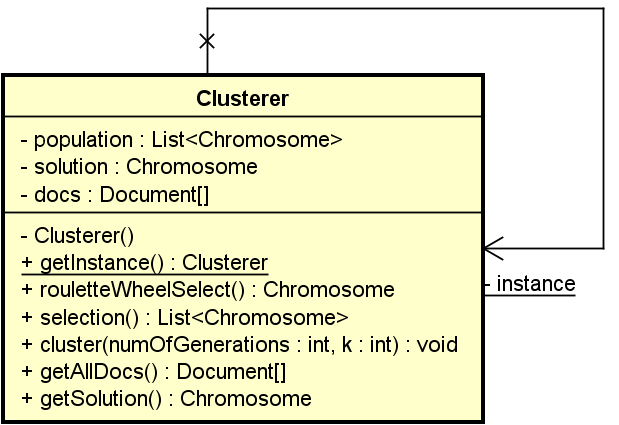
\includegraphics[width=0.5\textwidth]{DiagramKelas/Clusterer}
		\caption{Kelas \textit{Clusterer}}
		\label{fig:kelasClusterer}
	\end{center}
\end{figure}

Kelas ini merupakan kelas utama yang akan mengatur jalannya proses pengelompokan. Kelas ini merupakan kelas singleton. Atribut yang terdapat dalam kelas ini adalah:

\begin{itemize}
	\item \textit{docs}: bertipe \textit{List of Document} yang berfungsi untuk menyimpan seluruh koleksi dokumen.
	\item \textit{instance}: variabel \textit{static} ini berfungsi untuk menyimpan \textit{instance} dari kelas \textit{Clusterer}.
	\item \textit{population}: bertipe \textit{List of Chromosome} yang merepresentasikan populasi pada generasi saat ini.
	\item \textit{solution}: bertipe \textit{Chromosome} yang mencatat kromosom dengan nilai \textit{fitness} terbaik.
\end{itemize}

\textit{Method} yang terdapat dalam kelas ini adalah:

\begin{itemize}
	\item \textit{Clusterer}: merupakan \textit{constructor private} yang berfungsi untuk menjamin tidak akan ada \textit{instance} dibuat diluar dari kelas ini.
	\item \textit{getInstance}: merupakan \textit{getter} dari variabel \textit{instance}.
	\item \textit{rouletteWheelSelect}: bertugas untuk memilih dua kromosom dan melakukan persilangan untuk menghasilkan sebuah keturunan selanjutnya.
	\item \textit{selection}: bertugas untuk melakukan \textit{roulette wheel selection} sebanyak populasi untuk menghasilkan populasi dari generasi selanjutnya.
	\item \textit{cluster}: merupakan \textit{method} utama yang bertugas melakukan pengelompokan dokumen dengan dua parameter yaitu jumlah generasi dan nilai $k$.
	\item \textit{getAllDocs}: merupakan \textit{getter} dari atribut \textit{docs}.
	\item \textit{getSolution}: merupakan \textit{getter} dari atribut \textit{solution}.
\end{itemize}

\begin{figure}
	\begin{center}
		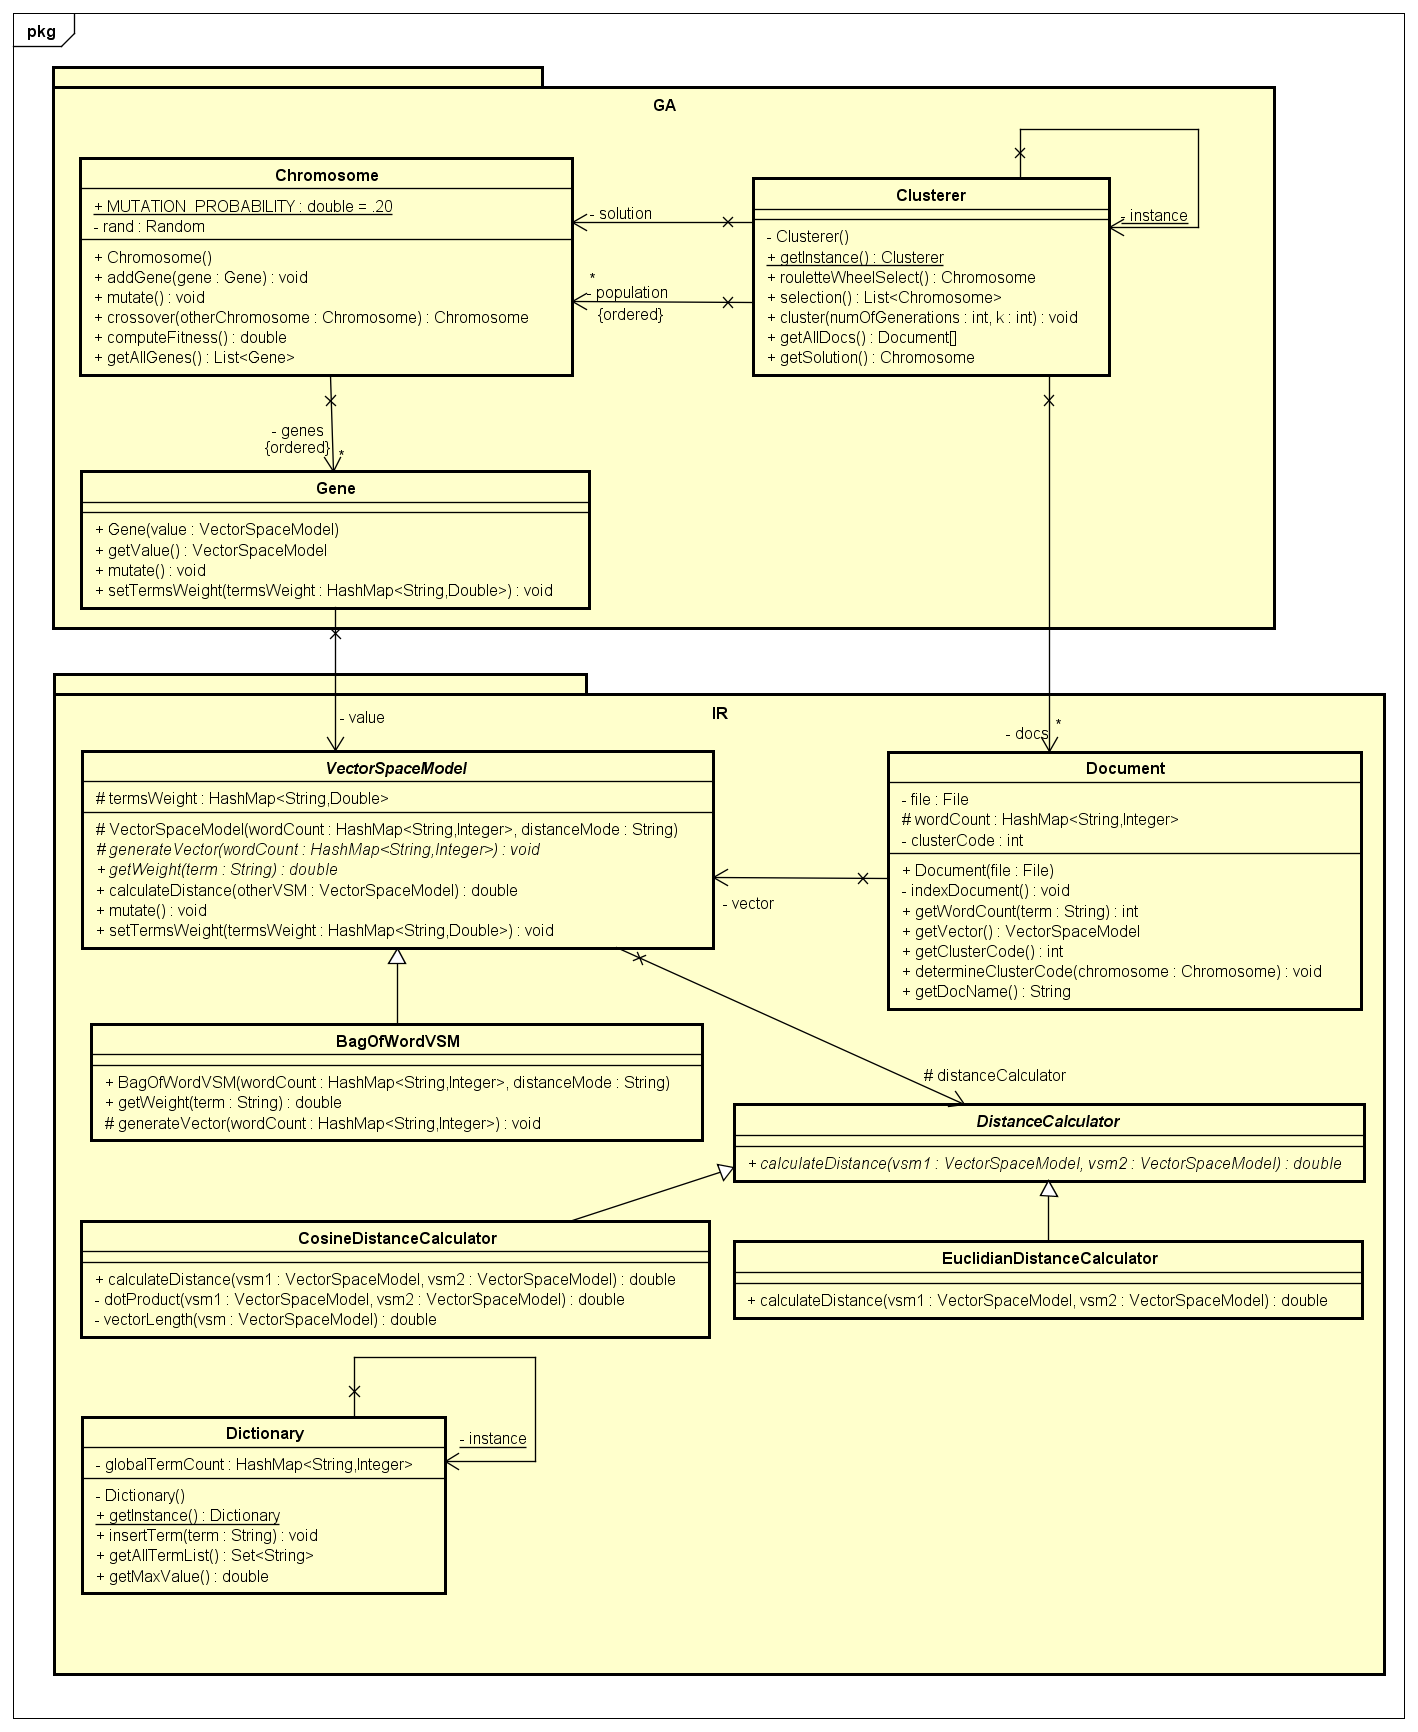
\includegraphics[width=\textwidth]{DiagramKelas}
		\caption{Diagram kelas pada tahap perancangan}
		\label{fig:diagramkelas}
	\end{center}
\end{figure}

\newpage

\section{Perancangan Antarmuka Pengguna}
Antarmuka yang dirancang untuk perangkat lunak ini hanya terdiri dari satu jendela utama dan dua jendela \textit{pop-up}. Pada penelitian ini, perancangan antarmuka dibuat menggunakan perangkat lunak \textit{balsamiq}\footnote{https://balsamiq.com/}. Setiap objek dan \textit{field} akan diberi label unik agar dapat disesuaikan dengan tabel keterangan. Berikut akan dibahas rancangan antarmuka pengguna dari perangkat ini.

\subsection{Jendela Utama}
Gambar \ref{fig:UIUtama} merupakan jendela yang pertama kali ditampilkan saat perangkat lunak dijalankan. Jendela tersebut berisi berbagai macam hal yang dibutuhkan penguna dalam melakukan pengelompokan dokumen. 

\begin{figure}[h]
	\begin{center}
		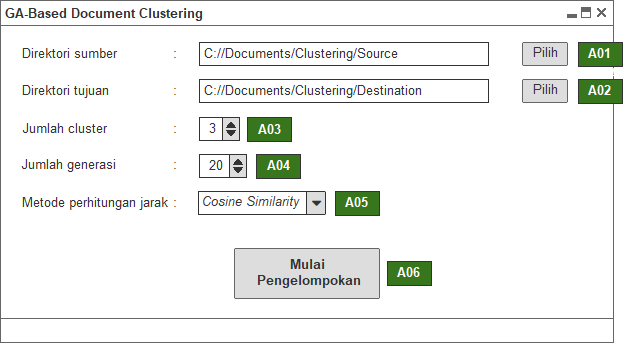
\includegraphics[width=0.7\textwidth]{UI/Main}
		\caption{Rancangan antarmuka jendela utama}
		\label{fig:UIUtama}
	\end{center}
\end{figure}

Penjelasan setiap \textit{field} dalam jendela utama adalah sebagai berikut:

\begin{table}[h]
	\label{tbl:fieldUtama}
	\renewcommand{\arraystretch}{2}
	\begin{tabularx}{\textwidth}{l X l X l X} \hline
		\textbf{Kode} & \textbf{Nama} & \textbf{Jenis} & \textbf{\textit{Defaut value}} & \textbf{Wajib} & \textbf{Aturan validasi} \\ \hline
		A01 & Direktori sumber & \textit{file chooser} & - & ya & Harus berupa direktori yang berisi dokumen (tidak boleh kosong) \\ \hline
		A02 & Direktori tujuan & \textit{file chooser} & - & ya & Harus berupa direktori yang kosong \\ \hline
		A03 & Jumlah cluster & \textit{spinner} & 2 & ya & Nilai minimum 2 \\ \hline
		A04 & Jumlah generasi & \textit{spinner} & 1 & ya & Nilai minimum 1 \\ \hline
		A05 & Metode perhitungan jarak & \textit{dropdown} & \textit{Cosine Similarity} & ya & - \\ \hline
	\end{tabularx}
	\caption{Rincian \textit{field} pada jendela utama}
\end{table}

Jendela ini hanya memiliki sebuah tombol dengan kode \textbf{A06} yang berfungsi untuk memulai proses pengelompokan dan membuka jendela \textit{loading}. Selain tombol, pada jendela ini juga terdapat lima \textit{field} seperti yang tertera pada Tabel \ref{tbl:fieldUtama}.

\subsection{Jendela \textit{Loading}}

\begin{figure}[h]
	\begin{center}
		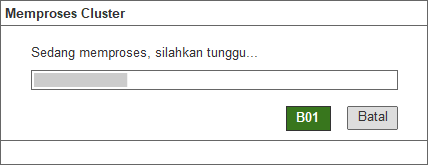
\includegraphics[width=0.7\textwidth]{UI/LoadingPage}
		\caption{Rancangan antarmuka jendela \textit{loading}}
		\label{fig:UILoading}
	\end{center}
\end{figure}

Gambar \ref{fig:UILoading} merupakan jendela yang akan muncul setelah pengguna menekan tombol "Mulai Pengelompokan". Jendela ini berisi informasi perkembangan proses pengelompokan. Informasi ini disajikan dalam bentuk \textit{progress bar}. Hanya ada sebuah tombol pada jendela ini yaitu tombol dengan kode \textbf{B01}. Sesuai dengan labelnya, tombol ini berfungsi untuk membatalkan proses pengelompokan. Apabila tombol batal ditekan, maka pengguna akan dikembalikan ke jendela utama (Gambar \ref{fig:UIUtama}).

\subsection{Jendela Proses Berhasil}
\begin{figure}[h]
	\begin{center}
		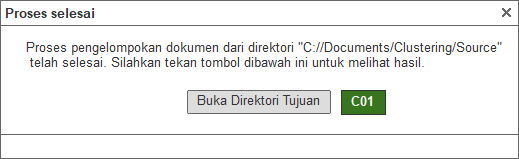
\includegraphics[width=0.7\textwidth]{UI/Output}
		\caption{Rancangan antarmuka jendela proses berhasil}
		\label{fig:UISuccess}
	\end{center}
\end{figure}

Gambar \ref{fig:UISuccess} akan ditampilkan setelah proses pengelompokan berhasil, yaitu saat \textit{progress bar} di jendela \textit{loading} sudah terisi penuh. Jendela ini hanya memiliki satu buah tombol yaitu tombol dengan kode \textbf{C01} yang berfungsi untuk membuka \textit{Windows Explorer} pada direktori hasil yang sudah dipilih pengguna pada jendela utama untuk menampilkan hasil dari proses pengelompokan.